\documentclass[paper=a4, fontsize=11pt]{scrartcl} 
\usepackage[utf8]{inputenc}
\usepackage{amsmath}
\usepackage{amsfonts}
\usepackage{amssymb}
\author{Kim Thuong Ngo}
\usepackage[T1]{fontenc} 
\usepackage{fourier} 
\usepackage{lipsum} 
\usepackage{listings}
\usepackage{graphicx}
\usepackage{tabularx}
\usepackage{sectsty}
\usepackage{xcolor}
\usepackage{wasysym}
\usepackage{stmaryrd}
\allsectionsfont{\centering \normalfont\scshape} 
\usepackage{fancyhdr} 
\usepackage{cancel}
\pagestyle{fancyplain} 
\fancyhead{}
\fancyfoot[L]{} 
\fancyfoot[C]{} 
\fancyfoot[R]{\thepage} 
\renewcommand{\headrulewidth}{0pt} 
\renewcommand{\footrulewidth}{0pt}
\setlength{\headheight}{13.6pt}

\numberwithin{equation}{section} 
\numberwithin{figure}{section} 
\numberwithin{table}{section}

\setlength\parindent{0pt}  

\newcommand{\horrule}[1]{\rule{\linewidth}{#1}} 

\title{	
\normalfont \normalsize 
\textsc{InformatikI} \\ [25pt] 
\horrule{0.5pt} \\[0.4cm] 
\huge Skript \\ 
\horrule{2pt} \\[0.5cm] 
}

\author{Kim Thuong Ngo} 
\date{\normalsize\today} 
\usepackage{color}
\definecolor{mygray}{rgb}{0.83,0.83,0.83}
\lstset{
   basicstyle=\small,
   keywordstyle=\color{orange},
   identifierstyle=,
   commentstyle=\color{Bittersweet},
   stringstyle=\ttfamily,
   breaklines=true,
   numbers=left,
   numberstyle=\small,
   frame=single,
   backgroundcolor=\color{mygray}
}
\usepackage{tikz}
\newcommand\circlearound[1]{%
  \tikz[baseline]\node[draw,shape=circle,anchor=base] {#1} ;}
%----------------------------------------------------------------------------------------
\begin{document}
\maketitle 
\newpage
\tableofcontents
%----------------------------------------------------------------------------------------
\newpage
\section{Sprachebene: Die Macht der Abstraktion - Anfänger}
\subsection{Scheme: Ausdrücke, Auswertung und Abstraktion}
Programm: DrRacket \\


\includegraphics[width=5cm,height=5cm]{Racketlogo.png}

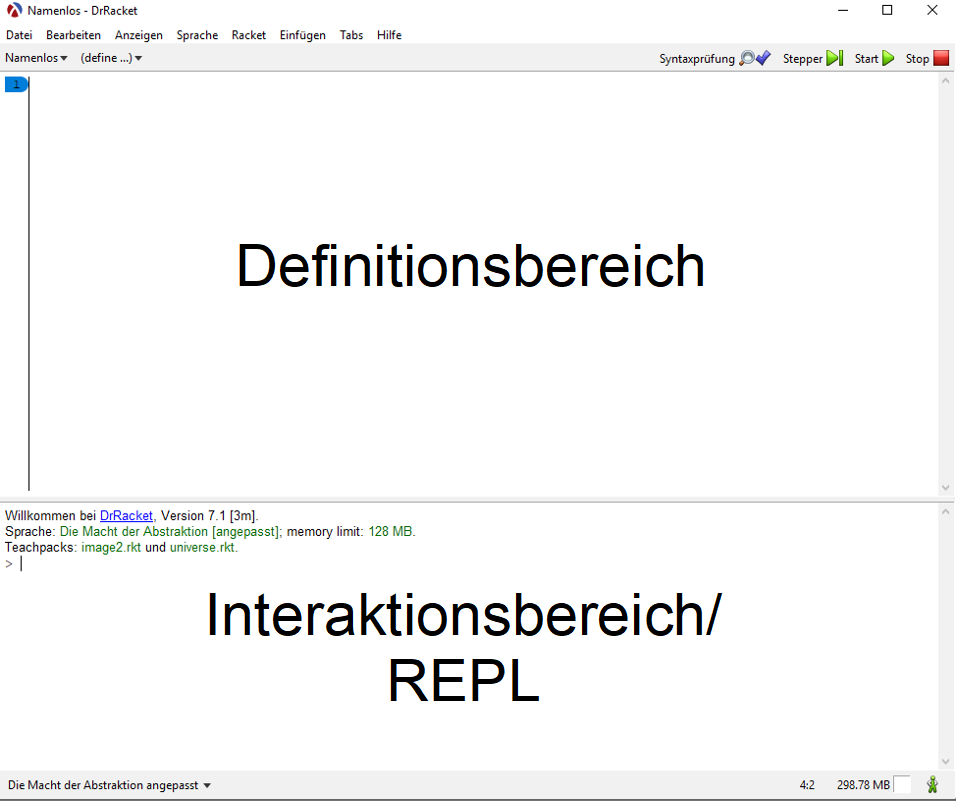
\includegraphics[width=10cm,height=8cm]{Racketfenster2.png}

Die Anwendung von Funktionen wird in Scheme \textcolor{orange}{ausschließlich} in \textcolor{orange}{Präfixnotation} durchgeführt: \\

\begin{tabular}{c|c}
Mathematik & Scheme \\\hline
$44-2$ & (- 44 2) \\
$f(x,y)$ & (f x y)\\
$\sqrt{81}$ & (sqrt 81)\\
$\lfloor x \rfloor$ & (floor x)\\
$9^{2}$  & (expt 9 2) \\
3! & (! 3) \\
\end{tabular}

Allgemein:
\begin{lstlisting}
(<function> <argument> ... <argument> )
\end{lstlisting}

(+ 40 2) und (odd? 42) sind Beispiele für \textcolor{orange}{Ausdrücke}, die bei der \textcolor{orange}{Auswertung} einen Wert liefern.

Notation: $\rightsquigarrow$ \\
\begin{tabular}{cc}
(+ 40 2) $\rightsquigarrow$ 42 & Auswertung/ Evaluation \\
(odd? 42) $\rightsquigarrow$ & Reduktion \\
\end{tabular}

Interaktionsfenster : Read $\rightarrow$ Evaluation $\rightarrow$ Print $\rightarrow$ Read $\rightarrow$ ... (REPL) \\

\textcolor{orange}{Literale} stellen für einen konstanten Wert (auch: \textcolor{orange}{Konstante}) und sind nicht weiter reduzierbar. \\
\begin{tabular}{cc|c}
Literal & & Signatur \\\hline
\# t \# f & Wahrheitswerte: true,false & boolean \\
" " "abc" "x" & Zeichenkette & string \\
007 0 1904 -42 & ganze Zahlen & integer \\
0 1 2 3 & natürliche Zahlen mit 0 & natural \\
-273.15 0.42 & Fließkommazahlen & real \\
$\dfrac{1}{2}$ $\dfrac{3}{4}$ & rationale Zahlen & rational \\
Bild & Bilder & image \\
\end{tabular}

Auswertung \textcolor{orange}{zusammengesetzter Ausdrücke} (composite expression) in mehreren Schritten (steps) "von innen nach außen", bis keine weitere Reduktion möglich ist. \\

(+ (+ 20 20) (+ 1 1)) $\rightsquigarrow$ (+ 40 (+ 1 1)) $\rightsquigarrow$ (+ 40 2) $\rightsquigarrow$ 42 \\

Beispiel: $0.7 + \dfrac{1}{2} / 0.25 - \dfrac{0.6}{0.3}$ \\

\textcolor{orange}{Achtung!} Scheme rundet bei Arithmetik mit Fließkommazahlen (interne Darstellung nicht präzise). Arithmetik mit rationalen Zahlen ist exakt. \\
Ein Wert kann an einen \textcolor{orange}{Namen} (identifier) \textcolor{orange}{gebunden} werden durch
\begin{lstlisting}
(define <id> <expression>)
\end{lstlisting}
Erlaubt konsistente Wiederverwendung und dient der Selbstdokumentation von Programmen. \\
\textcolor{orange}{Achtung!} Dies ist eine \textcolor{orange}{Spezialform} und kein Ausdruck. Insbesondere besitzt diese Spezialform keinen Wert, sondern einen Effekt: der Name  <id> wird an den Wert von <expression> gebunden. \\
Namen können in Scheme fast beliebig gewählt werden solange die Zeichen 
\begin{enumerate}
\item die Zeichen () {} [] " ´ `, ; | \# nicht vorkommen
\item der Name nicht einem numerischen Literal gleicht
\item kein whitespace 
\end{enumerate}
enthalten ist. \\
Beispiel: euro->US\$ \\
\textcolor{orange}{Achtung!} Groß- und Kleinschreibung ist im Identifier \textcolor{orange}{nicht} relevant. \\
Eine \textcolor{orange}{Lambda-Abstraktion} (auch Funktion oder Prozedur) erlaubt die Formulierung von Ausdrücken, in denen mittels \textcolor{orange}{Parametern} von konkreten Werten abstrahiert wird: 
\begin{lstlisting}
(lambda (<p1> <p2> ...) <expression>)
\end{lstlisting}
(lambda ... ) ist eine \textcolor{orange}{Spezialform}. Wert der Lambda-Abstraktion \# <procedure> \textcolor{orange}{Anwendung} (auch Applikation) der Lambda-Abstraktion führt zur Ersetzung aller Vorkommen der Parameter im Rumpf durch die angegebenen konkreten \textcolor{orange}{Argumente}: \\
Beispiel: ((lambda (days) (* days (* 155 minutes-in-a-day))) 365) $\rightsquigarrow$ (* 365 (* 155 minutes-in-a-day)) $\rightsquigarrow$ ... $\rightsquigarrow$ 81 468 000 \\

In Scheme leitet ein Semikolon ; einen \textcolor{orange}{Kommentar} ein, der bis zum Zeichenende reicht und von Racket bei der Auswertung ignoriert wird. Prozeduren und Funktionen sollten im Programm eine ein- bis zweizeilige \textcolor{orange}{Kurzbeschreibung} vorangestellt werden. \\

Eine \textcolor{orange}{Signatur} prüft, ob ein Name <id> an einen Wert einer angegebenen Sorte gebunden wird. Signaturverletzungen werden protokolliert.
\begin{lstlisting}
(: <id> <signatur>)
\end{lstlisting}

Bereits eingebaute Signaturen: 
\begin{itemize}
\item natural $\mathbb{N}_{0}$
\item integer $\mathbb{Z}$
\item rational $\mathbb{Q}$
\item real $\mathbb{R}$
\item number $\mathbb{C}$
\item boolean
\item string
\item image
\end{itemize}

\textcolor{orange}{Spezialform}, kein Wert \\

\textcolor{orange}{Prozedur-Signaturen} spezifizieren Signaturen sowohl für die Parameter <p1>,<p2>,... als auch für den Ergebniswert der Prozedur. 
\begin{lstlisting}
(: <id> (<signatur-p1> <signatur-p2> ... -> <signatur-ergebnis>))
\end{lstlisting}
Prozedur-Signaturen werden bei \textcolor{orange}{jeder} Anwendung der Funktion <id> auf Verletzung geprüft. \\

\textcolor{orange}{Testfälle} dokumentieren das erwartete Ergebnis einer Prozedur für ausgewählte Argumente.
\begin{lstlisting}
(check-expect <expression1> <expression2>)
\end{lstlisting}

Wertet Ausdruck <expression1> aus und teste, ob der erhaltene Wert der Erwartung (= Wert des Ausdrucks <expression2>) entspricht. Eine Prozedurdefinition sollten Testfälle direkt vorangestellt werden. \\
\textcolor{orange}{Spezialform}, keinen Wert, Testverletzungen werden protokolliert. \\

Konstruktionsformel für Prozeduren: 
\begin{enumerate}
\item Kurzbeschreibung (ein- bis zweizeiliger Kommentar, eingeleitet durch Semikolon ; )
\item Signatur (: <id> (... -> ...))
\item Testfälle check-epect/ check-within
\item Rumpf programmieren
\end{enumerate}
%---------------------------------------------------------------------------------------
\subsubsection{Top-Down-Entwurf}
Programmieren mit Wunschdenken \\

Beispiel: Sunset auf Tatooine (Star Wars IV) \\
Zeichne Szene zu Zeitpunkt t (t=0 ... 100) 
\begin{enumerate}
\item Himmel verfärbt sich
\item Sonne versinkt bei t=100
\item Luke starrt auf Horizont (bei jedem t)
\end{enumerate}
Zeichne Tatooine Sunset zu Zeitpunkt t
\begin{lstlisting}
(: tatooine (natural -> image))
(define tatooine
  (lambda (t)
     (overlay/pinhole (luke t)
                       (sun t)
                       (sky t))))
\end{lstlisting}

t=0: \\

\includegraphics[width=15cm,height=7cm]{tatooine0.png}

t=100: \\

\includegraphics[width=15cm,height=7cm]{tatooine100.png}
%---------------------------------------------------------------------------------------
\subsection{Reduktionsregeln für Scheme}
Fallunterscheidungen: je nach Ausdruck 
\begin{itemize}
\item Literale (1,\# t, "abc", ...) \\
         1 $\rightsquigarrow$ 1 (keine Reduktion möglich)
\item Identifier <id>\\
         <id> $\rightsquigarrow$ Wert \\
         Wert an den <id> gebunden ist [eval$_{id}$]
\item Lambda-Abstraktion \\
         (lambda (...) ...) $\rightsquigarrow$ (lambda (...) ...) [eval$_{\lambda}$]
\item Applikation                  
         \begin{enumerate}
         \item f, e1, e2, ... mittels $\rightsquigarrow$ erhalte f', e1', e2' , ...
         \item \begin{itemize}
                  \item Operation auf e1',e2',... falls f' primitive eingebaute Operation [apply$_{prim}$]
                  \item Argumentwerte e1',e2',... in Rumpf einsetzen, dann Rumpf mittels $\rightsquigarrow$ reduzieren falls f' Lambda-Abstraktion [apply$_{\lambda}$]         
                  \end{itemize}
         \end{enumerate}
\end{itemize}
Wiederhole Anwendungen von $\rightsquigarrow$ bis keine Reduktion mehr möglich ist. \\

Beispiele: 
\begin{enumerate}
\item (+ 40 2) \\
         $\rightsquigarrow^{eval_{id}, 2x eval_{lit}}$ (\# <procedure: +> 40 2) \\
         $\rightsquigarrow^{apply_{prim}}$ 42
\item (sqr 9) \\
         $\rightsquigarrow^{eval_{id},eval_{lit}}$ ((lambda (x) (* x x)) 9) \\
         $\rightsquigarrow^{apply_{\lambda}}$ (* 9 9) \\
         $\rightsquigarrow^{eval_{id}}$ (\# <procedure: *> 9 9) \\
         $\rightsquigarrow^{apply_{prim}}$ 81        
\end{enumerate}
%----------------------------------------------------------------------------------------
\subsubsection{Lexikalische Bindung}
Bezeichnen (lambda (x) (* x x)) und (lambda (r) (* r r)) die gleiche Funktion? \\
Antwort: JA \\
\textcolor{orange}{Achtung!}: Das hat EInfluss auf das korrekte Einsetzen von Argumenten für Parameter (siehe apply$_{\lambda}$) \\
Das \textcolor{orange}{bindende Vorkommen} eines Identifier <x> im Programmtext kann systematisch bestimmt werden:
\begin{enumerate}
\item (lambda (x) ...)
\item (define x ... )
\end{enumerate}
Prinzip der \textcolor{orange}{lexikalischen Bindung} \\
übliche Notation in der Mathematik: \textcolor{orange}{Fallunterscheidung!} \\

$$maximum(x_{1},x_{2}) = 
\begin{cases}
x_{1} & falls x_{1} \geq x_{2} \\
x_{2} & sonst
\end{cases}$$
%-------------------------------------------------------------------------------------------
\subsection{Fallunterscheidungen}
\textcolor{orange}{Tests} (auch: \textcolor{orange}{Prädikate}) sind Funktionen, die einen Wert der Signatur boolean liefern \\
Typische Primitive in Tests 
\begin{lstlisting}
(: = (number number -> boolean))
(: < (real real -> boolean))
(: string=? (string string -> boolean))
(: boolean=? (boolean boolean -> boolean))
(: zero? (number -> boolean))
\end{lstlisting}
weitere: odd?, even?, positive?, negative?, ...\\
\textcolor{orange}{Spezialform} Fallunterscheidung (conditional) 
\begin{lstlisting}
(cond (<test1> <expression>)
         (<t2> <e2)
         ...
         (<tn> <en>)
         (else <en+1>)) ; optional
\end{lstlisting}

Führt die Tests in der Reihenfolge <t1>,<t2>,... durch. Sobald <ti> zu #t ausgewertet, werte Zweig <ei> aus. <ei> ist das Ergebnis der Fallunterscheidung. Wenn <tn> #f liefert, dann liefere $\begin{cases} <en+1> \\ $Fehlermeldung: "cond. alle Tests ergaben #f" $\end{cases}$

Die Signatur \textcolor{orange}{one-of} lässt genau einen der n aufgezählten Werte zu.
\begin{lstlisting}
(one-of <e1> <e2> ... <en>)
\end{lstlisting}

Reduktion von cond [eval$_{cond}$] \\
\begin{itemize}
\item (cond (<t1> <e1>) (<t2> <e2>) ...)
         \begin{enumerate}
         \item Reduziere <t1>, erhalte <t1'>
         \item $\begin{cases}$
         <e1> falls <t1'> #t &  <t2>,<e2>,... werden \textcolor{orange}{nicht} ausgewertet \\
         (cond (<t2> <e2>) ... ) sonst & <e1> nicht ausgewertet
         $\end{cases}$
         \end{enumerate}
 \item (cond (else <en+1>)) $\rightsquigarrow$ <en+1>
 \item (cond) $\rightsquigarrow$ Fehler "cond, alle Tests ergaben \#f "        
\end{itemize}

\subsubsection{Binäre Fallunterscheidung}
\begin{lstlisting}
(if <t1> <e1> <e2>) = (cond (<t1> <e1>) (else <e2>))
\end{lstlisting}
%----------------------------------------------------------------------------------
\subsection{Zusammengesetzte Daten}
Daten können interessante interne Struktur (\textcolor{orange}{Komponenten}) aufweisen \\
Beispiel: ein Star Wars Charakter \\
\begin{tabular}{|cc|}
\hline
name & "Luke Skywalker" \\\hline
jedi? & \#f \\\hline
force & 25 \\\hline
... & \\\hline
\end{tabular}
\begin{lstlisting}
; Ein Charakter (character) besteht aus
; - Name (name)
; - Jedi Status (jedi?)
; - Stärke der Macht (force)
(define-record-procedures character
     make-character
     character?
     (character-name
     character-jedi?
     character-force))   
\end{lstlisting}

(make-character n j f) $\rightsquigarrow$ <Konstruktion> (siehe oben) \\
(character-name <Konstruktion>) $\rightsquigarrow$ n Selektor (Komponenten auslesen) \\
(character-jedi? <Konstruktion>) $\rightsquigarrow$ j \\
(character-force <Konstruktion>) $\rightsquigarrow$ f \\

\textcolor{orange}{Records} in Scheme \\
Record Definition legt fest 
\begin{itemize}
\item Record-SIgnatur (Name)
\item Konstruktor (baut aus Komponenten ein Record)
\item Prädikat
\item Liste von Selektoren (lesen je eine Komponente des Records)
\end{itemize}

\begin{lstlisting}
(define-record-procedures <t>
     make-<t>
     <t>?
     (<t>-<component1>
     ...
     <t>-<cn>))
\end{lstlisting}

Liste der Selektoren legt Komponenten (Anzahl, Reihenfolge, Name) fest. \\
Signatur des Konstruktors/ der Selektoren für Record-Signatur <t> mit n Komponenten <c1> ... <cn> 
\begin{lstlisting}
(: make-<t> (<t1> ... <tn> -> <t>))
                  ; n Komponenten Signaturen
(: <t>-<ci> (<t> -> <ti>))                  
\end{lstlisting}
$\forall$ string n, boolean, natural f: \\
(character-name (make-character n j f)) $\rightsquigarrow$ n \\
(character-jedi? (make-character n j f)) $\rightsquigarrow$ j \\
(character-force (make-character n j f)) $\rightsquigarrow$ f \\

Aussagen über die Interaktion von zwei (oder mehr) Funktionen: algebraische \textcolor{orange}{Eigenschaft}. \\

\textcolor{orange}{Spezialform} check-property
\begin{lstlisting}
(check-property
     (for-all ((<id1> <signatur1>)
                ...
                (<idn> <signaturn>))
      <expression>))      
      ; Prädikat, dass sich auf <id1> ... <idn> bezieht    
\end{lstlisting}
Test erfolgreich, falls <expression> für beliebige Bindungen für <id1> ... <idn> \textcolor{orange}{immer} \#t ergibt. \\
Interaktion von Konstruktor und Selektor 
\begin{lstlisting}
(for-all ((n string)
           (j boolean)
           (f natural))
(string=? (character-name
                   (make-character n j f)) n)))           
\end{lstlisting}
Beispiel: Die Summe zweier natürlicher Zahlen ist mindestens so groß wie jede dieser Zahlen. \\
$\forall x_{1},x_{2} \in \mathbb{N}: x_{1} + x_{2} \geq max(x_{1}, x_{2})$ 
\begin{lstlisting}
(check-property
     (for-all ((x1 natural)
                (x2 natural))
      (>= (+ x1 x2) (max x1 x2))))            
\end{lstlisting}

Konstruktion von Funktion f, die zusammengesetzte Daten der Signatur <t> \textcolor{orange}{konsumiert}. \\
Welche Record-Komponenten <ci> sind relevant für <f>? \\
\begin{lstlisting}
; Schablone
(: <f> (... <t ... -> ...))
(define <f>
   (lambda ( ... r ...) 
       ( ... <t>-<ci> r) ...)))
\end{lstlisting}

Prozedur <f> die zusammengesetzte Daten der Signatur <t> konstruiert/ produziert Konstruktoraufruf  für <t> \textcolor{orange}{muss} enthalten sein! 
\begin{lstlisting}
(: <f> ( ... -> <t>))
(define <f>
     (lambda (...)
          ( ... (make-<t> ...) ...)))
\end{lstlisting}

Sei <p> ein Prädikat mit Signatur (<t> -> boolean). \\ 
Eine Signatur (predicate <p>)  gilt für jeden Wert x mit Signatur <t> für den zusätzlich (<p> x) $\rightsquigarrow$ \#t gilt. \\
Signatur (predicate <p>) ist damit spezifischer (restriktiver) als Signatur <t>. \\
Einführung eines neuen Signaturnamens <new-t> für die Signatur <t>
\begin{lstlisting}
(define <new-t (signature <t>))
\end{lstlisting}
Beispiele:
\begin{lstlisting}
; Farbe einer Karte
(define farbe
     (signature (one-of "karo" "herz" "pik" "kreuz")))
     
; Breitengrad - latitude? ist ein Prädikat
(define latitude
     (signature (predicate latitude?)))     
\end{lstlisting}

Übersetze eine Ortsangabe mittels Google Geocoding \\
API in eine Position auf der Erdkugel 
\begin{lstlisting}
(: geocoder (string -> (mixed geocode geocode-error)))
\end{lstlisting}
Ein geocode besteht aus ... \\
\begin{tabular}{|c|c|}
\hline
 & Signatur \\\hline
Adresse (address) & string \\
Ortsangabe (loc) & location \\
Norostecke (northeast) & location \\
Südwestecke (southwest) & location \\
Typ (type) & string \\
Genauigkeit (accuracy) & string \\\hline 
\end{tabular}
%----------------------------------------------------------------------------------
\subsection{Gemischte Daten}
Die Signaturen \textcolor{orange}{mixed} (mixed <t1> ... <tn>) ist gültig für jeden Wert, der mindestens eine der Signaturen <t1> ... <tn> erfüllt. \\
Beispiel 1: Datendefinition \\
Die Antwort des Geocoders ist \textcolor{orange}{entweder} \\
\begin{itemize}
\item ein Geocode (Signatur geocode) \textcolor{orange}{oder} 
\item eine Fehlermeldung (Signatur geocode-error)
\end{itemize}
\begin{lstlisting}
(mixed geocode geocode-error)
\end{lstlisting}

Beispiel 2: (eingebaute Funktion string -> number) 
\begin{lstlisting}
(: string->number (string -> (mixed number (one-of #f))))
\end{lstlisting}
(string-> number "42") $\rightsquigarrow$ 42 \\
(string->number "fortytwo") $\rightsquigarrow$ \#f \\
Das Prädikat <t>? einer Record-Signatur <t> unterscheidet Werte der Signatur <t> von \textcolor{orange}{allen anderen } Werten:
\begin{lstlisting}
(: <t>? (any -> boolean))
\end{lstlisting}
Auch: Prädikate für eingebaute Signaturen \\
\begin{itemize}
\item number?
\item complex?
\item real?
\item rational?
\item integer?
\item natural?
\item string?
\item boolean?
\end{itemize}

Prozeduren, die gemischte Daten der Signaturen <t1> ... <tn> konsumieren 
\begin{lstlisting}
(: <f> ((mixed <t1> ... <tn>) -> ... ))
(define <f>
     (lambda (x)
          (cond
               ((<t1>? x) ... )
               ...
               ((<tn>? x) ... ))))
\end{lstlisting}
Mittels \textcolor{orange}{let} lassen sich Werte an \textcolor{orange}{lokale Namen} binden:
\begin{lstlistig}
(let ((<id1> <e1>)
      ...
      (<idn> <en>))
  <e>)    
\end{lstlisting}
Die Ausdrücke <e1> ... <en> werden \textcolor{orange}{parallel} ausgewertet. \\
$\Rightarrow$ <id1> ... <idn> können in <e> (\textcolor{orange}{und nur dort!} verwendet werden. \\
Der Wert des let-Ausdrucks ist der Wert von <e> \\
nur dort: \begin{itemize}
\item Verwendung nur in <e>, nicht in den <ei>!
\item lokal: Verwendung nicht außerhalb des (let ... )
\end{itemize}
\textcolor{orange}{Achtung!} Sprachlevel: Die Macht der Abstraktion 
\begin{lstlisting}
; syntaktischer Zucker

(let ((<id1> <e1>)
       ...
       (<idn> <en>))
   <e>)

((lambda          (<id1> ... <idn>) <e>)
    <e1> ... <en>)
\end{lstlisting}
(check-error <e> <message>) erwartet Programmabbruch mit Fehlermeldung <msg>. \\
Erzwingen des Programmabbruchs mittels 
\begin{lstlisting}
(violation <msg>)
\end{lstlisting}
%----------------------------------------------------------------------------------
\subsection{Polymorphe Signaturen}
Beobachtung: Manche Prozeduren arbeiten unabhängig von den Signaturen ihrer Argumente \textcolor{orange}{parametrisch polymorphe Prozeduren} (griech. vielgestaltig). \\
Nutze \textcolor{orange}{Signaturvariablen} \\
Beispiel:
\begin{lstlisting}
; Identität
(: id (%a -> %a))
(define id (lambda (x) x))

; konstante Funktion (ignoriert 2. Argument)
(: const (%a %b -> %a))
(define const (lambda (x y) x))

; Projektion (ein Argument auswählen)
(: proj ((one-of 1 2) %a %b -> (mixed %a %b)))
(define proj 
     (lambda (i x y) 
          (cond
               ((= i 1) x)
               ((= i 2) y))))
\end{lstlisting}

Beachte: Parametrisch polymorphe Prozeduren "wissen nichts" über ihre Argumente mit Signatur \%a,\%b,... und können diese \textcolor{orange}{nur} reproduzieren oder zu andere polymorphe Prozeduren weiterreichen \\
Eine polymorphe Signatur steht für alle Signaturen, in denen die Signaturvariablen \textcolor{orange}{konsistent} durch konkrete Signaturen ersetzt werden. \\
Beispiel: Wenn eine Prozedur (\%a number \%b -> \%a) erfüllt, dann auch
\begin{lstlisting}
(string number boolean -> string)
(boolean number boolean -> boolean)
(string number natural -> string)
(number number number -> number)
\end{lstlisting}
%----------------------------------------------------------------------------------
\subsection{Polymorphe Paare und Listen}
\begin{lstlisting}
; ein polymorphes Paar (pair) besteht aus
; - erste Komponente (first)
; - zweite Komponente (rest)
; wobei die Komponenten beliebige Werte sind
(define-record-procedures-parametric pair pair-of
      make-pair
      pair?
      (first
      rest))
\end{lstlisting}

(pair-of <t1> <t2>) ist eine Signatur für Paare deren erste und zweite Komponente von der Signatur <t1> bzw. <t2> sind.

\begin{lstlisting}
(: make-pair (%a %b -> (pair-of %a %b)))

(: first ((pair-of %a %b) -> %a))
(: rest ((pair-of %a %b) -> %b))
\end{lstlisting}

Eine \textcolor{orange}{Liste} von Werten der Signatur <t>, (list-of <t>), ist entweder \\
\begin{itemize}
\item leer (Signatur empty-list) oder
\item ein Paar (Signatur pair-of) aus
        \begin{itemize}
        \item einem Listenkopf (Signatur <t>) und
        \item einer Restliste (Signatur (list-of <t>)
        \end{itemize}
\end{itemize}

\begin{lstlisting}
(define list-of
     (lambda (t)
          (signature (mixed empty-list
                                     (pair-of t (list-of t))))))
\end{lstlisting}

(list-of <t>) Listen, deren Elemente die Signatur <t> besitzen \\
Signatur empty-list bereits in Racket vordefiniert \\
ebenfalls vordefiniert
\begin{lstlisting}
(: empty empty-list)
(: empty? (any -> boolean))
\end{lstlisting}
%--------------------------------------------------------------------
\subsubsection{Visualisierung von Listen}
\begin{lstlisting}
(make-pair 1
                (make-pair 2
                                empty))
\end{lstlisting}

$\lightning$ Notation skaliert schlecht \\
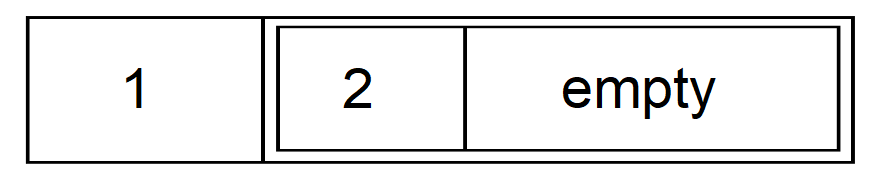
\includegraphics[width=8cm,height=5cm]{Listen.png}

\textcolor{orange}{Spines} (Rückgrat) \\
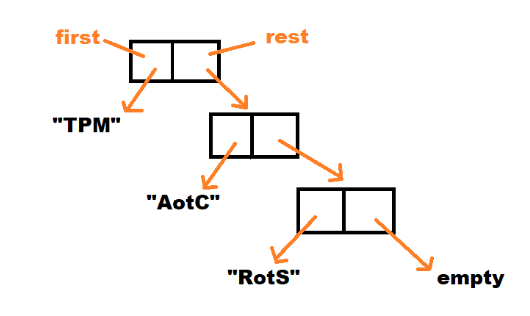
\includegraphics[width=10cm,height=7cm]{spine1.png}
% ----------------------------------------------------------------------
\subsubsection{Prozeduren über Listen}
Schablonen für gemischte und zusammengesetzte Daten \\
Beispiel:
\begin{lstlisting}
(: list-sum ((list-of umber) -> number))

(check-expect (list-sum empty) 0)
(check-expect (list-sum (make-pair 40
                                                    (make-pair 2
                                                                    empty))) 42)
                                                                    
(define list-sum
      (lambda (xs)
           (cond
               ((empty? xs) 0)
               ((pair? xs) (+ (first xs)
                                    (list-sum (rest xs)))))))                                                                    
\end{lstlisting}

Schablone für Funktion <f>, die Liste xs konsumiert
\begin{lstlisting}
(: <f> ((list-of <t1>) -> <t2>))

(define <f>
     (lambda (xs)
          (cond
               ((empty? xs) ... )
               ((pair? xs) ... (first xs)
                               ... (<f> (rest xs)) ... ))))
\end{lstlisting}
%---------------------------------------------------------------------------------
\section{Neue Sprachebene: Die Macht der Abstraktion}
\begin{itemize}
\item Signatur (list-of $\%a$) eingebaut
\item neuer syntaktischer Zucker eingebaut
\end{itemize}

\begin{lstlisting}
(list <e1> <e2> ... <en>)
=
(make-pair <e1>
               (make-pair <e2>
                                ...
                                (make-pair <en>
                                                empty)))
\end{lstlisting}
Ausgabeformat für nicht leere Listen \\
\# <list <e1> <e2> ... <en>> \\

Füge Listen xs, ys zusammen (con\textcolor{orange}{cat}enate) \\
2 Fälle (xs leer oder nicht leer) \\
\begin{tabular}{cccc}
1) & $\overbrace{empty}^{xs}$ & $\overbrace{y_{1} y_{2} ... y_{m}}^{ys} $& $\overbrace{\vspace{10 mm} y_{1} y_{2} ... y_{m}}^{(cat xs ys) }$
2) &  $x_{1} x_{2} ... x_{n}$ & $y_{1} y_{2} ... y_{m}$ & $\underbrace{\underbrace{x_{1}}_{(first xs)} $ $\underbrace{ x_{2} ... x_{n}}_{(rest xs} \underbrace{y_{1} y_{2} ... y_{m}}_{ys} }_{(cat (rest xs) ys)} $
\end{tabular}

Bemerkungen: \\
\begin{itemize}
\item die Länge von xs (hier n) bestimmt die Anzahl der rekursiven Aufrufe
\item auf ys werden keine Selektoren angewandt
\end{itemize}
%----------------------------------------------------------------------------------
\subsection{match}
\textcolor{orange}{Spezialform match} \\
vergleicht einen Wert <e> mit gegebenen \textcolor{orange}{Patterns} <pat1> <pat2> ... <patn> \\
Falls <pati>, $1 \leq i \leq n$, das erste Pattern ist, das auf <e> matched, ist Zweig <ei> das Ergebnis (ansonsten wir die Auswertung mit "keiner der Zweige passte" abgebrochen
\begin{lstlisting}
(match <e>
   (<pat1> <e1>)
   (<pat2> <e2>)
   ...
   (<patn> <en>))
\end{lstlisting}

\textcolor{orange}{Pattern Matching} \\
\begin{enumerate}
\item Literal <l> \\
         <e> matched, falls <e> $\rightsquigarrow$ <l>
\item Don't Care _ \\
         <e> matched immer
\item Variable <v> \\        
         <e> matched immer, danach ist <v> an den Wert von <e> in <ei> gebunden
\item Record Konstruktor (<c> <pat1> ... <patk>) $k \geq 0$ \\
        <e> matched, wenn es durch (<c> <x1> ...  <xk>) konstruiert und <xj> auf <patj> matched, $1 \leq j \leq k$  \\
        \textcolor{orange}{Achtung!} Fall 4 ermöglicht Pattern Matching auf komplex konstruierten Werten       
\end{enumerate}
%---------------------------------------------------------------------------------
\subsection{Rekursion über natürliche Zahlen}
Die natürlichen Zahlen (vgl. gemischte Daten) \\
Eine natürliche Zahl (natural) ist entweder \\
\begin{itemize}
\item die Null 0 (zero)
\item die Nachfolger (succ) einer natürlichen Zahl $\mathbb{N}= {0, (succ 0), (succ (succ 0)), ...}$
\end{itemize}
Konstruktoren \\
\begin{lstlisting}
(: zero natural)
(define zero 0)

(: succ (natural -> natural))
(define succ
    (lambda (n)
        (+ n 1)))
\end{lstlisting}

Bedingte algebraische Eigenschaften (siehe check-property) \\
(... $\underbrace{<p>}_{Prädikat}$ $ \underbrace{<e>}_{Ausdruck}$) \\
Nur wenn <p> $\rightsquigarrow$ \#t, wird der Ausdruck <e> ausgewertet und getestet, ob <e> $\rightsquigarrow$ \#t \\
Beispiel: Fakultätsfunktion $n! (n \in \mathbb{N})$: \\
$0! = 1$ \\
$n! = n * (n-1)! \equiv (succ n)! = (succ n) * n!$ \\

$3! = 3*2! = 3* (2 * 1!) = 3*(2*(1*0!)) = 3*(2*(1*1)) =6$ \\

\begin{lstlisting}
; Berechne n!
(: factorial (natural -> natural))
(define factorial
    (lambda (n)
         (cond
             ((zero? n) 1)
             (else (* (factorial (- n 1)) n)))
             
(define factorial2
     (lambda (n)
          (cond
              ((= n 0) 1)
              (else (* (factorial (- n 1)) n)))             
\end{lstlisting}

Schablone für Funktionen <f>, die natürliche Zahl konsumieren:
\begin{lstlisting}
(: <f> (natural -> <t>))
(define <f>
    (lambda (n)
        (cond
            ((= n 0) ...)
            ((> n 0) ... (<f> (- n 1)) ... )))
\end{lstlisting}
SATZ \\
Eine Funktion, die nach der Schablone für Listen oder natürliche Zahlen geschrieben ist, \textcolor{orange}{terminiert immer} (= liefert immer ein Ergebnis) \\

Reduktion kann durchaus zur Konstruktion von Ausdrücken führen, die zunehmende Größe aufweisen (für factorial bestimmt das Argument die Größe) \\

Wenn möglich erzeuge Reduktionsprozesse, die \textcolor{orange}{konstanten Platzverbrauch} - unabhängig von Funktionsargumenten - benötigen \\

Beobachtung: \\
(Assoziativität von Multiplikation) \\
(* 10 (* 9 (* 8 ( * 7 (* 6 (factorial 5)))))) \\
= (* (* (* (* (* 10 9) 8) 7) 6) (factorial 5)9 \\
= (* 30240 (factorial 5)) \\
$\Rightarrow$ Multiplikation kann verzogen werden \\

Idee: \\
Führe Multiplikationen jeweils sofort aus \\
Schleife das Zwischenergebnis (\textcolor{orange}{akkumulierendes Argument}) durch die Berechnung \\
am Ende enthält der Akkumulator das Endergebnis \\

Berechne 5! \\
\begin{tabular}{c|c}
n & acc \\\hline
5 & 1 \\
4 & 5 \\
3 & 20 \\
2 & 60 \\
1 & 120 \\
0 & 120 \\
\end{tabular} 

\begin{lstlisting}
; worker
(: fac-worker (natural natural -> natural))
(define fac-worker
    (lambda (n acc)
        (cond
            ((= n 0) acc)
            ((> n 0) (fac-worker (- n 1) (* acc n))))))
            
; wrapper
(: fac (natural -> natural))
(define fac
     (lambda (n)
         (fac-worker n 1)))            
\end{lstlisting}

Ein Reduktionsprozess ist \textcolor{orange}{iterativ}, falls seine Größe konstant bleibt. \\
Damit ist factorial nicht iterativ, aber fac-worker ist iterativ \\

Wieso ist fac-worker iterativ? \\
Der rekursive Aufruf ersetzt den aktuell reduzierten Ausdruck \textcolor{orange}{vollständig}. Es gibt keinen \textcolor{orange}{Kontext} (ungebundenen Ausdruck), der auf das Ergebnis des rekursiven Aufrufs "wartet" \\
Kontext des rekursiven Aufrufs \\
\begin{itemize}
\item factorial (* n /hbox)
\item fac-worker -keiner-
\end{itemize}

Ein Prozeduraufruf ist \textcolor{orange}{endrekursiv}, wenn er keinen Kontext besitzt \\
Prozeduren, die nur endrekursive Prozeduraufrufe enthalten, heißen selbst endrekursiv. \\
Endrekursive Prozeduren führen zu iterativen Reduktion \\

Beobachtung: Berechnung von (rev (from-to 1 1000)) \\
$\overbrace{(cat \underbrace{(list 1000 999 ... 2)}_{\underbrace{(cat (list 1000 999 ... 3) (list 2 1)}_{999 Aufrufe von make-pair}} (list 1))}^{1000 Aufrufe von make-pair} $\\

$\Rightarrow$ Anzahl der Aufrufe von make-pair: $1000+999+...+1$ \\
rev auf einer Liste der Länge n \\
$\sum^{n}_{i=n}= \dfrac{1}{2} * n * (n+1)$ quadratisch in n \\

Konstruiere iterative Listenumkehr (backwards) \\
Berechnung von (backwards (list 1 2 3)) \\

\begin{lstlisting}
(: backwards-worker ((list-of %a) (list-of %a) -> (list-of %a)))
\end{lstlisting}

\begin{tabular}{c|c}
xs & acc \\\hline
(list 1 2 3) & empty \\
(list 2 3) & (list 1) \\
(list 3) & (list 2 1) \\
empty & (list 3 2 1) 
\end{tabular}
%----------------------------------------------------------------------------------
\subsection{letrec}
Mittels \textcolor{orange}{letrec} lassen sich Werte an \textcolor{orange}{lokale Namen} binden
\begin{lstlisting}
(letrec ((<id1> <e1>)
            ...
            <idn> <en>))
   <e>)         
\end{lstlisting}
Die Ausdrücke <e1> ... <en> dürfen selbst auf die Namen <id1> ... <idn> beziehen. Der Wert des gesamten letrec-Asudrucks ist der Wert von <e>.
%----------------------------------------------------------------------------------
\subsection{Induktive Definitionen}
Konstruktive Definition der natürlichen Zahlen \mathbb{N} \\
\textcolor{orange}{Definition (Peano Axiome)} \\
\begin{tabular}{|c|c|}
\hline
P1 & $0 \in \mathbb{N}$ (Null) \\\hline
P2 & $\forall n \in \mathbb{N}: succ(n) \in \mathbb{N}$ (Nachfolger) \\\hline
P3 & $\forall n \in \mathbb{N}: succ(n) \neq 0$ \\\hline
P4 & $\forall m,n \in \mathbb{N}: succ(m) = succ(n) \Rightarrow m=n$ \\\hline
P5 & $\mathbb{N}$ enthält nicht mehr als 0 und die durch die succ() generierte Elemente \\
     & nichts sonst ist in $\mathbb{N}$ 
     & \textcolor{orange}{Induktsionsaxiom} \\
     & für jede Menge $M \subseteq \mathbb{N}$: \\
     & Falls $0 \in M $ und $\forall n : (n \in M \Rightarrow succ(n) \in M)$, dann ist $M= \mathbb{N}$\\\hline
\end{tabular}
\includegraphics[width=5cm,height=5cm]{NatürlicheZahlen.png}
%------------------------------------------------------------
\subsubsection{Beweisschema der vollständigen Induktion}
Sie P(n) ist eine Eigenschaft einer Zahl $n \in \mathbb{N}$ (Prädikat) \\
\begin{lstlisting}
(: P (natural -> boolean))
\end{lstlisting}
Ziel: Zeige $\forall n \in \mathbb{N}: P(n) $ \\
Definiere: $M:= {n \in \mathbb{N}| P(n) gilt} \subseteq \mathbb{N}$ \\
\textcolor{orange}{Induktionsaxiom P5 für M } \\
 Falls $0 \in M $ und $\forall n : (n \in M \Rightarrow succ(n) \in M)$, dann ist $M= \mathbb{N}$ \\
 \textcolor{orange}{\fbox{Falls P(0) und $\forall n: (P(n) \Rightarrow P(succ(n))$, dann $\forall n \in \mathbb{N: P(n)}$}}
 
 Beispiel 1: \\
 $1= 1$ \\
 $1+3 = 4$ \\
 $1+3+5= 9$ \\
 $1+3+5+7 = 16$ \\
 $ [ \underbrace}\sum^{n}_{i=0}(2i+1)}_{$Summer der ersten n+1 ungeraden natürlichen Zahlen}=(n+1)^{2}$ ] \equiv P(n)$ \\
 
 Zeige:  $\forall n \in \mathbb{N}: P(n)$ \\
 Induktionsbasis P(0) \\
 $\sum^{0}_{i=0}(2i+1)=2*0+1=1=(0+1)^{2}$ \\
 Induktionsschritt $\forall n: P(n) = P(n+1)$ \\
 $\sum^{n+1}_{i=0}(2i+1)=\sum^{n}_{i=0}+2*(n+1)+1$ \\
 $=^{I.V.} (n+1)^{2} +2n+3 = n^{2}+4n+4 = (n+2)^{2}$ \\
 
 \hfill \box
 
 Beispiel 2: \\
 \begin{lstlisting}
 (define factorial
      (lambda (k)
            (if (= k 0)
                 1
                 (* k (factorial (- k 1))))))
 \end{lstlisting}
 $P(n) \equiv [(factorail n) = n!]$ \\
 Zeige: $\forall n \in \mathbb{N}: P(n)$ \\
 Induktionsbasis P(0) \\
 (factorial 0) \\
 $\rightsquigarrow$ ((lambda (k) ...) 0) \\
 $\rightsquigarrow$ (if (= 0 0) 1 ...) \\
 $\rightsquigarrow$ (if \#t 1 ...) \\
 $\rightsquigarrow$ 1=0! \\
 Induktionsschritt $\forall n: (P(n) \Rightarrow P(n+1))$ \\
 (factorial (n+1)) \\
 $\rightsquigarrow$ ((lambda (k) ...) n+1) \\
 $\rightsquigarrow$ (if (= n+1 0) ... (* ... )) \\
 $\rightsquigarrow$ (if #f ... (* ...)) \\
 $\rightsquigarrow$ (* n+1 (factorial (- n+1 1))) \\
 $\rightsquigarrow$ (* n+1 (factorial n)) \\
 $=^{I.V.}$ (* n+1 n!) = (n+1)!
 
 \hfill \box
 
 Annahme: - realisiert Differenz korrekt, * realisiert Multiplikation korrekt \\
 
 Beispiel \\
 Jedes f, das sich an die Schablone für Funktionen über natürliche Zahlen hält liefert immer ein Ergebnis (terminiert immer) \\
 
 Sei f also definiert durch:
 \begin{lstlisting}
 (: f (natural -> %a))
 (define f
     (lambda (n)
         (if (= n 0)
             basis
             (step (f (- n 1)) n))))
             
; Bemerkung
(: basis %a)                          ; Ausdruck             
(: step (%a natural -> %a))   ; totale Funktion
 \end{lstlisting}
 Dann gilt: $P(n) \equiv $ f(n) terminiert mit Ergebnis der Signaur $\%a$ \\
 
 Beweis: \\
 Induktionsbasis P(0) \\
 f(0) \\
 $\rightsquigarrow$ (if (= 0 0) basis ...) \\
 $\rightsquigarrow$ (if #t basis ...) \\
 $\rightsquigarrow$ basis \\
 Induktionsschritt $\forall n:(P(n) \Rightarrow P(n+1))$ \\
 (f n+1) \\
 $\rightsquigarrow$ (if (= n+1 0) ... (step ... )) \\
 $\rightsquigarrow$ (if #f ... (step ... )) \\
 $\rightsquigarrow$ (step (f (- n+1 1)) n+1) \\
 $\rightsquigarrow$ (step $\underbrace{(f n)}_{$terminiert mit EIgenschaft R$}$ (n+1))\\
 $\rightsquigarrow$ (step R n+1) terminiert
 
 \hfill \box
 
 %-------------------------------------------------------------
 \subsubsection{Definition Listen}
 die Menge M* (= listen mit Elementen aus M (list-of M)) ist induktiv definiert \\
 \begin{tabular}{cc}
 L1 & empty $\in$ M*\\
 L2 & $\forall x \in m, xs \in M*$:(make-pair x xs) $\in $ M* \\
 L3 & \nichts sonst ist in M*\\
 \end{tabular}
 \textcolor{orange}{Schema für Listeninduktion} \\
 Sei P(xs) eine Eigenschaft von Listen über M: 
 \begin{lstlisting}
 (: P ((list-of M) -> boolean))
 \end{lstlisting}
 
 Falls P(empty) Induktionsanfang bzw. Induktionsbasis ud $\forall x \in M, xs \in M*: (P(xs) \Rightarrow $ P((make-pair x xs))) Induktionsschritt, dann $\forall xs \in M*: P(xs)$ \\
 
 Beispiel: Eigenschaften von cat und append
\begin{lstlisting}
(define cat
    (lambda (xs ys)
        (cond
            ((empty? xs) ys)
            ((pair? xs) (make-pair (first xs)
                                             (cat (rest xs) ys))))))
\end{lstlisting}

\begin{tabular}{ccc}
1 & (cat empty ys) & ys\\
2 & (cat xs empty) & xs \\
3 & (cat (cat xs ys) zs) & (cat xs (cat ys zs)) \\
\end{tabular}
 
 (M*, cat, empty) ist ein Monoid \\
 
 Beweis: \\
 % TODO 
 \hfill \box
 
 Beispiel: Interaktion von length und cat
\begin{lstlisting}
(define length
   (lambda (xs)
       (cond
           ((empty? xs) 0)
           ((pair? xs) (+ 1 (length (rest xs)))))))
\end{lstlisting}

$ys \in M*$ sei beliebig \\
$P(xs) \equiv$ (length (cat xs ys)) = (+ (length xs) (length ys)) \\

Beweis: \\ 
Induktionsbasis P(empty): \\

Induktionsschritt

%Todo

\hfill \box
%----------------------------------------------------------------------------------
\subsection{Prozeduren höherer Ordnung (Higher Order Procedures HOP)}
Abstraktion von Funktionsparameter \\
\begin{lstlisting}
; extrahiere die Elemente xs, die das Prädikat p? erfüllen
(: filter ((%a -> boolean) (list-of %a) -> (list-of %a)))

(define filter
   (lambda (p? xs)
       (cond
           ((empty? xs) empty)
           ((pair? xs) (if (p? (first xs))
                                (make-pair (first xs)
                                                 (filter p? (rest xs))
                                 (filter p? (rest xs)))))))                 
\end{lstlisting}

Prozeduren höherer Ordnung (Higher Order Procedures kurz. HOP) \\
\begin{enumerate}
\item akzeptieren Prozeduren als Parameter und/oder 
\item liefern eine Prozedur als Ergebnis
\end{enumerate}

$\Rightarrow$ filter ist vom Typ1 \\

HOP vermeiden Duplizierung von Code und führen zu: \\
\begin{itemize}
\item kompaktere Programme
\item verbesserte Lesbarkeit
\item verbesserte Wartbarkeit
\end{itemize}

%------------------------------------------------------------------
\subsubsection{map}
Beispiel: (map f xs)

%todo zeichnung spine

\begin{lstlisting}
; wende f auf alle Elemente von xs an
(: map ((%a -> %b) (list-of %a) -> (list-of %b))

(define map
    (lambda (f xs)
        (cond
            ((empty? xs) empty)
            ((pair? xs) (make-pair (f (first xs))
                                             (map f (rest xs)))))))
\end{lstlisting}

\textcolor{orange}{Hinweis} \\
Verwende einfache Lambda-Abstraktion direkt als \textcolor{orange}{anonyme} Funktion. Wenn eine globale Benennung (via define) nicht gerechtfertigt erscheint. (z.B. lokaler/ einmaliger Benutzung) \\

%------------------------------------------------------------------
\subsubsection{Listenfaltung (fold)}
Allgemeine Transformation von Listen \textcolor{orange}{Listenfaltung (list folding)} \\
Idee: die Listenkonstruktoren und empty werden systematisch ersetzt: \\

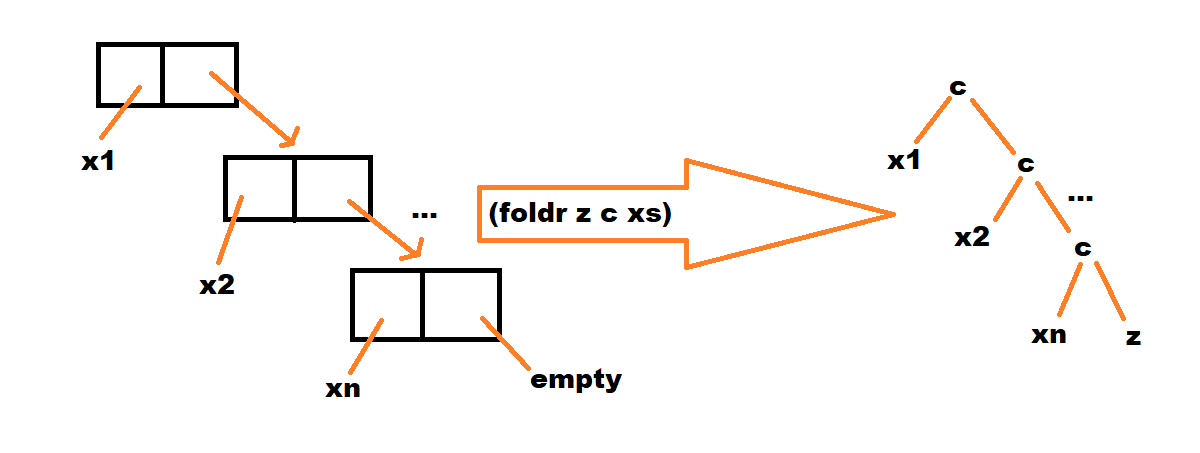
\includegraphics[width=15cm,height=8cm]{foldr.png}

(foldr z c xs) wirkt als Spine Transformer \\
\begin{itemize}
\item empty $\rightarrow$ z
\item make-pair $\rightarrow$ c
\end{itemize}

Eingabe: Liste (list-of $\%a$) \\
Ausgabe: im allgemeinen \textcolor{orange}{keine} Liste (etwa $\%b$)

\begin{lstlisting}
(: foldr (%b (%a %b -> %b) (list-of %a) -> %b))

(define foldr
   (lambda (z c xs)
        (cond
           ((empty? xs) z)
           ((pair? xs) (c (first xs)
                               (foldr z c (rest xs)))))))
\end{lstlisting}

Beispiel: Reduktion von xs \\
Multiplikation \\
\begin{lstlisting}
(: foldr-mult ((list-of number) -> number)))
(define foldr-mult
    (lambda (xs)
         (foldr 1 * xs)))
\end{lstlisting}
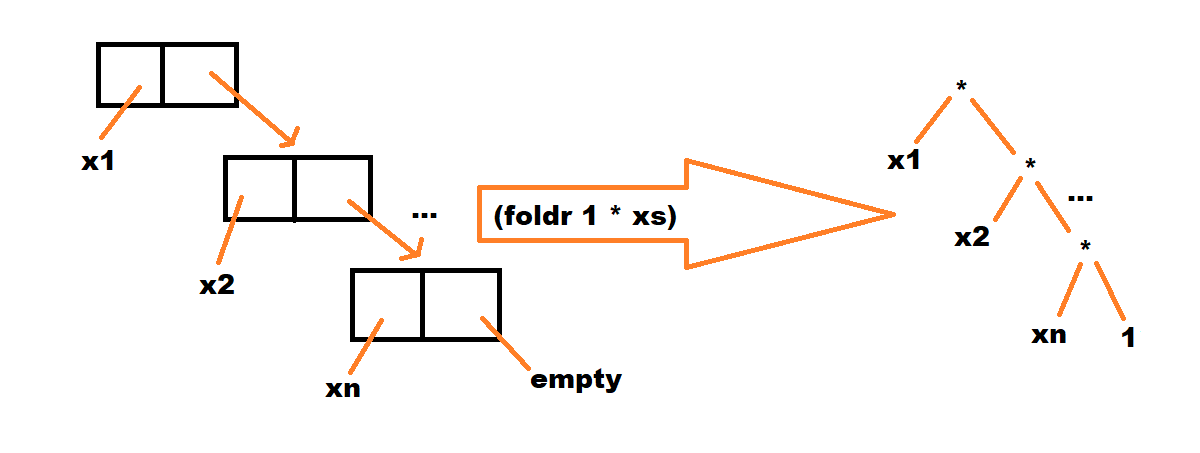
\includegraphics[width=15cm,height=8cm]{foldr_Multiplikation.png}

Summe \\
\begin{lstlisting}
(: sum ((list-of number) -> number)))
(define sum
    (lambda (xs)
         (foldr 0 + xs)))
\end{lstlisting}
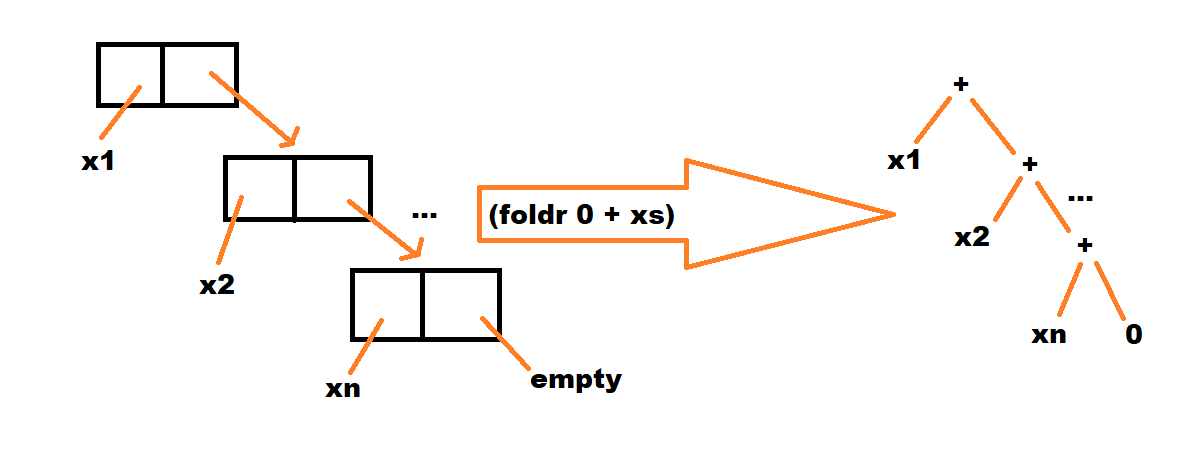
\includegraphics[width=15cm,height=8cm]{foldr_Summe.png}

Listenlänge \\
\begin{lstlisting}
(: list-length ((list-of %a) -> number)))
(define list-length
    (lambda (xs)
         (foldr 0 (lambda (y ys) (+ 1 ys)) xs)))
\end{lstlisting}
\includegraphics[width=15cm,height=8cm]{foldr_Listenlänge.png}

Spine Transformation \\
\begin{itemize}
\item empty $\rightarrow$ 0
\item (make-pair y ys) $\rightarrow$ (lambda (y ys) (+ 1 ys))
\end{itemize}

Teachpack "universe" nutzt HOP, um Animation (= Sequenzen von Szenen / Bildern) zu definieren \\
\begin{lstlisting}
(big-bang <init>
               (on-tick <tock>)
               (to-draw <render> <w> <h>))
\end{lstlisting}

\begin{itemize}
\item (: <init> $\%a$) \\
         Startzustand
\item (: <tock> ($\%a$ -> $\%a$)) \\
         Funktion, die neuen aus alten Zustand berechnet, wird 28 Mal/Sekunde aufgerufen
\item (: <render> ($\%a$ -> image)) \\
         Funktion, die aus aktuellen Zustand eine Szene berechnet (wird in Fenster mit <w>x<h> Pixeln angezeigt)
\item beim Schließen der Animation wird der letzte aktuelle Zustand zurückgegeben
\end{itemize}
%----------------------------------------------------------------
\subsubsection{Komposition von Funktionen (allgemein)}

((compose f g) x) $\equiv$ (f (g x)) \\
Mathematik: (compose f g) $\equiv f \circ g$ "f nach g" \\
$\Rightarrow$ compose konstruiert aus f und g eine \textcolor{orange}{neue Funktion} ("Funktionsfabrik") \\

\begin{lstlisting}
(: compose ((%b -> %c) (%a -> %b) -> (%a -> %c)))

(define compose
     (lambda (f g)
        (lambda (x)
            (f (g x)))))
\end{lstlisting}

repeat: n-fache Komposition einer Funktion f mit sich selbst \\
(n-fache Anwendung von f, Exponentiation): \\
\begin{itemize}
\item $f^{0} = id$ (Identität id $\equiv$ (lambda (x) x)
\item $f^{n} = f^{n-1} \circ f$
\end{itemize}

\begin{lstlisting}
(: repeat (natural (%a -> %a) -> (%a -> %a)))

(define repeat
    (lambda (n f)
        (cond
            ((= n 0) (lambda (x) x))
            ((> n 0) (compose (repeat (- n 1) f) f)))))
            
; greife auf das n-te Element von xs zu (n > 0)
(: nth (natural (list-of %a) -> %a))

(define nth 
    (lambda (n xs)
         ((compose first (repeat (- n 1) rest)) xs)))            
\end{lstlisting}

%-----------------------------------------------------------------
\subsubsection{Currying}
Reduktion von ((add 1) 41) \\
$\rightsquigarrow^{eval(id)}$ (((lambda (x) (lambda (y) (+ x y))) 1) 41) \\
$\rightsquigarrow^{apply \lambda (\lambda x)}$ ((lambda (y) (+ 1 y)) 41) \\
$\rightsquigarrow^{apply \lambda (\lambda y)}$ (+ 1 41) \\
$\rightsquigarrow^{apply, prim(\lambda)}$ 42

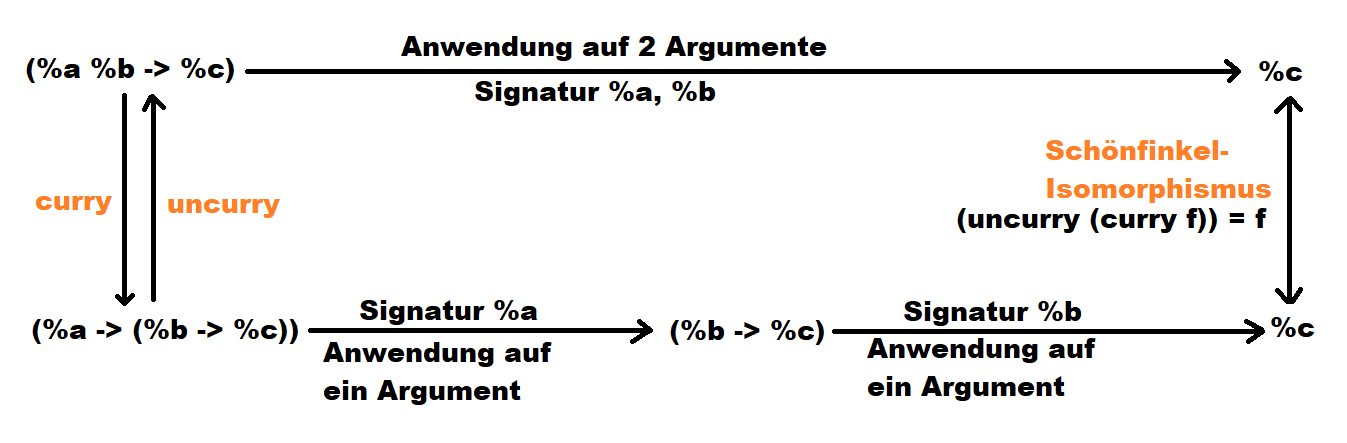
\includegraphics[width=15cm,height=8cm]{currying.png}

\begin{itemize}
\item Currying (Haskell B. Curry, Moses Schönfinkel) \\
        Anwendung einer Funktion auf ihre erstes Argument liefert ein Funktion der restlichen Argumente 
\item jede n-stellige Funktion lässt sich in eine alternative \textcolor{orange}{curried} Variante transformieren, die in n-Schritten jeweils nur ein Argument konsumiert: curry
\end{itemize}

\begin{lstlisting}
(: curry ((%a %b -> %c) -> (%a -> (%b -> %c))))
(define curry
     (lambda (f)
         (lambda (x y)
                  ((f x) y)))))
                  
(: uncurry ((%a -> (%b -> %c)) -> (%a %b -> %c)))
(define uncurry
   (lambda (f)
        (lambda (x)
             (lambda (y)
                  (f x y))))                
\end{lstlisting}        

Erinnerung: Bestimmung der ersten Ableitung der reellen Funktion f durch Bildung des \textcolor{orange}{Differnzenquotienten}:

% todo: graph

$\dfrac{f(x+h)-f(x)}{h}$ Differenzenquotient \\

$lim_{h \rightarrow 0} \dfrac{f(x+h)-f(x)}{h} = f'(x)$ Differentialquotient \\

Operator ' (Ableitung) konsumiert FUnktion f und produziert f' \\
$\Rightarrow$ ' ist higher order \\
%-----------------------------------------------------------------
\subsection{Streams}
\begin{lstlisting}
(stream-of %a)
\end{lstlisting}
\textcolor{orange}{unendliche} Ströme von Elementen x, der Signatur $\%a$ \\
Ein Stream ist ein Paar \\

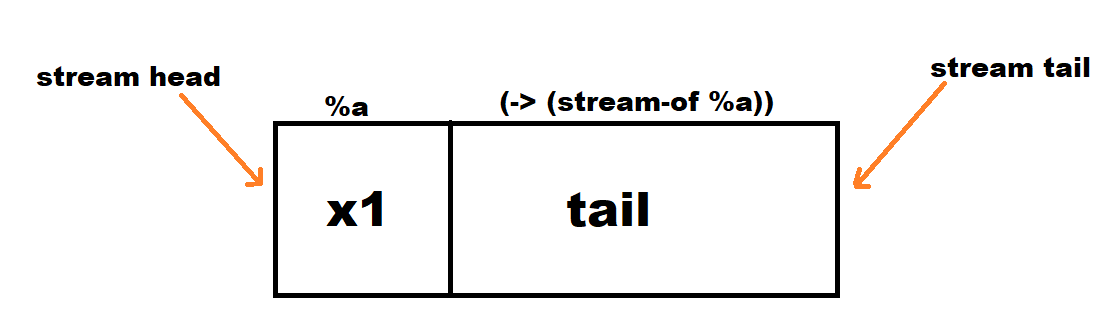
\includegraphics[width=15cm,height=8cm]{streams.png}

Vergleiche: \\
\begin{tabular}{cc}
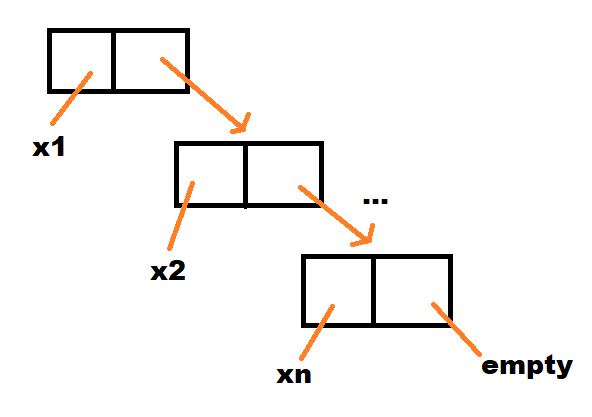
\includegraphics[width=7cm,height=5cm]{Listendarstellung.png} & 
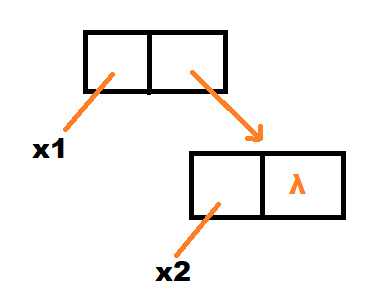
\includegraphics[width=7cm,height=5cm]{Streamdarstellung.png}
\end{tabular}

Verzögerte Auswertung eines Ausdrucks (delayed evaluation):
\begin{lstlisting}
(: delay (%a -> (-> %a)))
\end{lstlisting}

(delay <e>): verzögere die Auswertung des Ausdrucks <e> und liefere "Versprechen" (promise) , <e>  bei Bedarf später auswerten zu können \\
\textcolor{orange}{Implementation}\\
(delay <e>) $\equiv$ (lambda () <e>) \\
(force <p>): Erzwinge Auswertung des Promise <p>, liefere den Wert des verzögerten Ausdrucks \\

\begin{lstlisting}
(: force ((-> %a) -> %a))
(define force
    (lambda (p) (p)))
\end{lstlisting}

%------------------------------------------------------------------
\subsubsection{Sieb des Eratosthenes}
(Generierung \textcolor{orange}{aller} Primzahlen; Stream-Programm über 200 Jahre alt) \\
\begin{enumerate}
\item starte mit dem Stream str der Zahlen 2,3,4,...
\item Die erste Zahl n im str ist eine Primzahl
\item Streiche alle Vielfachen von n im Stream str
\item weiter bei 2.
\end{enumerate}

\textcolor{orange}{\circlearound{2}}
\textcolor{orange}{\circlearound{3}} \cancel{4} 
\textcolor{orange}{\circlearound{5}} \cancel{6} 
\textcolor{orange}{\circlearound{7}} \cancel{8} \cancel{9} \cancel{10} 
\textcolor{orange}{\circlearound{11}} \cancel{12} 
\textcolor{orange}{\circlearound{13}} \cancel{14} \cancel{15} \cancel{16} 
\textcolor{orange}{\circlearound{17}} \cancel{18} 
\textcolor{orange}{\circlearound{19}} \cancel{20} \cancel{21} \cancel{22} 
\textcolor{orange}{\circlearound{23}} \cancel{24} \cancel{25} \cancel{26} \cancel{27} \cancel{28} 
\textcolor{orange}{\circlearound{29}} \cancel{30} ...

%-----------------------------------------------------------------------
\subsection{Binärbäume}
Die Menge der \textcolor{orange}{Binärbäume} T(M) über M ist induktiv definiert: \\
\begin{tabular}{cc}
T1 & empty-tree $\in$ T(M) \\\
T2 & $\forall x \in M,l,r \in T(M)$: (make-node l x r) $\in$ T(M)\\
T3 & Nichts sonst ist in T(M)\\
\end{tabular}

Hinweise: \\
\begin{itemize}
\item Jeder Knoten (made-node) in einem Binärbaum hat 2 \textcolor{orange}{Teilbäume} l und r sowie eine \textcolor{orange}{Markierung} (\textcolor{orange}{label}) $x \in M$
\item vgl. M* und T(M) \\
        empty-list und empty-tree \\
        make-pair und make-node
\end{itemize}

Visualisierung und Terminologie \\
\begin{itemize}
\item empty-tree: \box
\item (make-node l x r): 
\item der Knoten mit Markierung x ist \textcolor{orange}{Wurzel} (\textcolor{orange}{root}) des Baumes
\item ein Knoten, der nur leere Teilbäume besitzt, heißt \textcolor{orange}{Blätter} \\
         alle anderen Knoten sind \textcolor{orange}{innere Knoten} (\textcolor{orange}{inner nodes})         
\end{itemize}

Beispiele für Binärbäume der Menge T($\mathbb{N}$) \\
Baum T1: listenartig (rechtstief) \\
\begin{itemize}
\item Knoten mit Label 1 ist \textcolor{orange}{Wurzel}
\item Knoten 3 ist \textcolor{orange}{Blatt}
\item Knoten 1,2 sind \textcolor{orange}{innere Knoten}
\end{itemize}

\begin{tikzpicture}[level/.style={sibling distance=60mm/#1}]
\node [circle,draw] (z){$1$}
  child {node [circle,draw] (a) {}
  }
  child {node [circle,draw] (j) {$2$}
    child {node [circle,draw] (k) {}}
    child {node [circle,draw] (l) {$3$}
        child {node [circle,draw] (m) {}}
        child {node [circle,draw] (n) {}}
    }
 }
\end{tikzpicture}

Baum T2: balanciert \\
\begin{itemize}
\item Knoten 1 ist \textcolor{orange}{Wurzel} und \textcolor{orange}{innerer Knoten}
\item Knoten 2,3 sind \textcolor{orange}{Blätter}
\end{itemize}

\begin{tikzpicture}[level/.style={sibling distance=60mm/#1}]
\node [circle,draw] (z){$1$}
  child {node [circle,draw] (a) {$2$}
    child {node [circle,draw] (b) {}}
    child {node [circle,draw] (g) {}}
  }
  child {node [circle,draw] (j) {$3$}
    child {node [circle,draw] (k) {}}
  child {node [circle,draw] (l) {}}
}
\end{tikzpicture}

(Binär-)Bäume haben zahllose Anwendungen \\
\begin{itemize}
\item Suchbäume (schneller Zugriff, z.B. Datenbanksysteme)
\item Datenkompressionen
\item Darstellung von Programmen/ Ausdrücken im  Rechner
\item ...
\end{itemize}

Bäume sind \textcolor{orange}{DIE} induktive Datenstruktur der Informatik! \\

%-----------------------------------------------------------
\subsubsection{Tiefe eines Baumes}
Die \textcolor{orange}{Tiefe} (\textcolor{orange}{depth}) eines Binärbaumes t ist die maximale Länge eines Weges von der Wurzel bis zu einem leeren Teilbaum \\
\begin{tabular}{|c|c|}
\hline
(btree-depth empty-tree) & 0 \\\hline
(btree-depth T2) & 2 \\\hline
(btree-depth T1) & 3 \\\hline
(btree-depth classifier) & 4 \\\hline
\end{tabular}

Schablone (gemischte + zusammengesetzte Daten) \\

\begin{lstlisting}
(: btree-depth ((btree-of %a) -> natural))

(define btree-depth
    (lambda (t)
        (cond
           ((empty-tree? t) 0)
           ((node? t) (+ 1 (max (btree-depth (node-left-branch t))
                                           (btree-depth (node-right-branch t))))))))
\end{lstlisting}

%--------------------------------------------------
\subsubsection{Pretty Printing}
Einschub: Pretty Printing von Binärbäume \\
Prozedur (pp <t>) erzeugt formatierte String Binärbäume <t> \\

% todo bilder

Idee: Repräsentiere formatierenden String als \textcolor{orange}{Liste von Zeilen (String)} \\
\begin{enumerate}
\item Nutze (string-append ...) um Zeilen-Strings zu definieren (horizontal)
\item Nutze (append ...) um die einzelnen Zeilen zu einer Liste von Zeilen zusammen zu setzen (vertikal)
\end{enumerate}
Erst direkt vor der Ausgabe werden die Zeilen Strings zu einem auszugebenden String zusammengesetzt (strings-list>string)

%-----------------------------------------------------
\subsubsection{Induktion über Binärbäume}
Sei P(t) eine Eigenschaft von Binärbäumen $t \in T(M)$, also 
\begin{lstlisting}
(: P ((b-tree-of M) -> boolean))
\end{lstlisting}
Falls P(empty-tree) [Induktionsbasis] und $\forall x \in M,l,r \in T(m): P(l) \wedge P(r) \Rightarrow$ P((make-node l x r)) [Insuktionsschritt] dann $\forall t \in T(M): P(t)$ \\

Beispiel: Zusammenhang zwischen Größe (btree-size) und Tiefe (btree-depth) eines Binärbaumes t: \\

$P(t) \equiv (btree-depth t) \leq (btree-size t) \leq 2^{(btree-depth t)} -1$ \\

Induktionsbasis: P(empty-tree)

Induktionsschritt: $P(l) \wedge P(r) \Rightarrow$ P((make-node l x r))
% todo
\hfill /box

%------------------------------------------------
\subsubsection{Tree-Transformer}
Erinnerung: fold ist Spine-Transformer üfr Liste xs

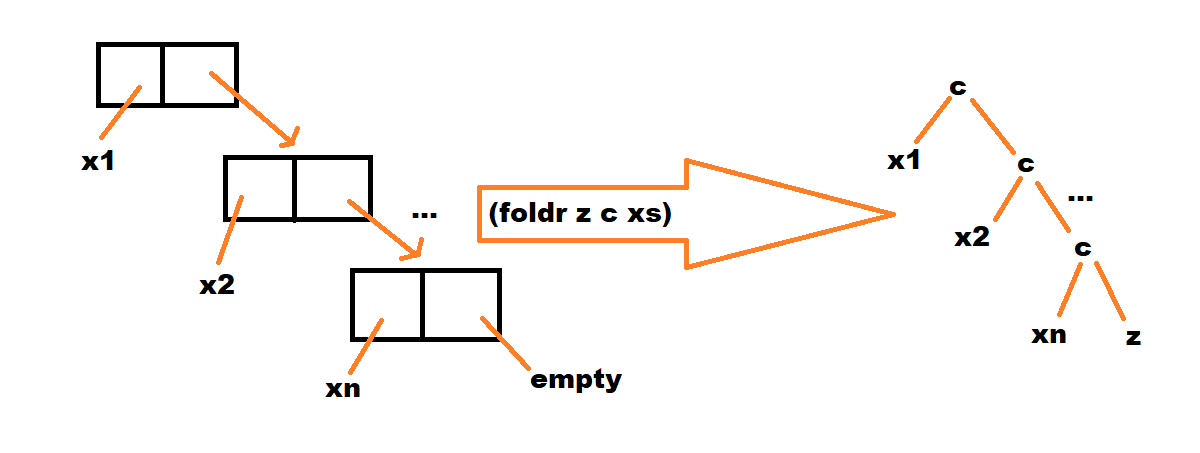
\includegraphics[width=15cm,height=8cm]{foldr.png}

Wie müsste btree-fold, eine fold-Operation für Binärbäume, verhalten? \\

Tree-Transformer für Bäume t:

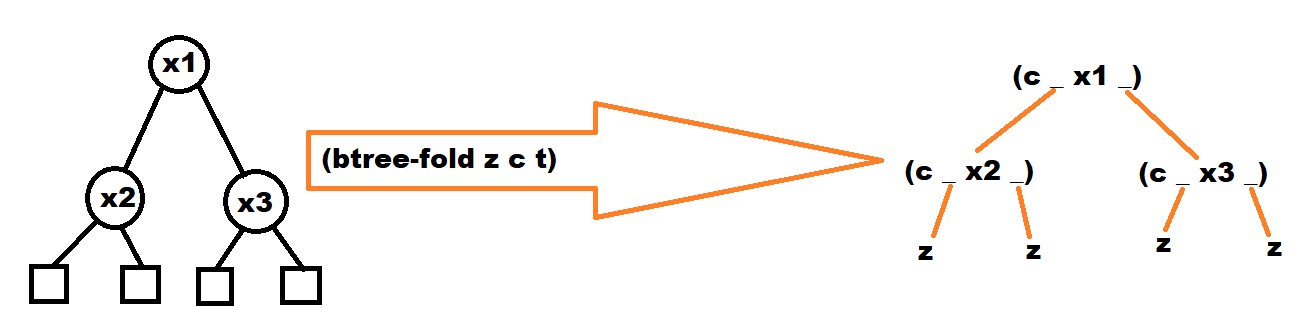
\includegraphics[width=15cm,height=8cm]{btree-fold.png}

\begin{lstlisting}
; falte Baum bzgl. z und c
(: btree-fold (%b (%b %a %b -> %b) (btree-of %a) -> %b)))

(define btree-fold
    (lambda (z c t)
        (cond
            ((empty-tree? t) z)
            ((node? t) (c (btree-fold z c (node-left-branch t))
                                 (node-label t)
                                 (btree-fold z c (node-right-branch t)))))))
\end{lstlisting}

Beispiel: Bestimme die Markierung lm \textcolor{orange}{links-außen} im Baum t (oder empty, falls t leer ist) \\

% todo graph

\begin{lstlisting}
(: leftmost ((btree-of %a) -> (list-of %a)))
(define leftmost
    (lambda (t)
        (btree-fold empty
                         (lambda (l1 x l2)
                              (if (empty? l1) (list x) l1))
                         t)))     
\end{lstlisting}
%-----------------------------------------------------
\subsubsection{Baumdurchläufe}
Ein \textcolor{orange}{Tiefendurchlauf} (depth-first-traversal) eines Baumes t sammelt die Markierungen jedes Knoten n in t auf. Die markierungen der Teilbäume l,r des Knotens n=(make-node l x r) werden \textcolor{orange}{vor} x eingesammelt (Durchlauf zuerst in der Tiefe) \\
Je nachdem, ob x (a) zwischen, (b) vor, (c) nach den Markierungen von l,r eingeordnet wird, erhält man ein \\
\begin{tabular}{|c|c|c|}
\hline
(a) & \textcolor{orange}{inorder} traversal & 1 2 3 \\\hline
(b) & \textcolor{orange}{preorder} traversal & 2 1 3 \\\hline
(c) & \textcolor{orange}{postorder} traversal & 1 3 2 \\\hline
\end{tabular}

\begin{lstlisting}
(: inorder ((btree-of %a) -> (list-of %a)))
(define inorder
    (lambda (t)
        (btree-fold empty
                         (lambda (xs1 x xs2)
                             (append xs1 (list x) xs2))
                          t)))   
\end{lstlisting}

Beispiel: Baumdarstellung des arithmetischen Ausdrucks (Term)
$$2+\underbrace{3*4}_{* bindet stärker +}$$

Daher:

\begin{tikzpicture}[level/.style={sibling distance=60mm/#1}]
\node [circle,draw] (z){$+$}
  child {node [circle,draw] (a) {$2$}
    child {node [circle,draw] (b) {}}
    child {node [circle,draw] (g) {}}
  }
  child {node [circle,draw] (j) {$*$}
    child {node [circle,draw] (k) {$3$}
        child {node [circle,draw] (m) {}}
        child {node [circle,draw] (n) {}}}
    child {node [circle,draw] (l) {$4$}
        child {node [circle,draw] (o) {}}
        child {node [circle,draw] (p) {}}}}
}
\end{tikzpicture}

Ein \textcolor{orange}{Breitendurchlauf} (breath-first-traversal) eines Baumes t sammelt die Markierungen der Knoten \textcolor{orange}{ebenenweise}  vo der Wurzel ausgehend auf: \\

\includegraphics[width=10cm,height=8cm]{levelorder.png}

(levelorder t) $\rightsquigarrow$ (list "s" "c" "h" "e" "m" "e") \\

Idee: gegeben sei eine Liste ts von Bäumen \\
\begin{enumerate}
\item Sammle die Liste der Markierungen der Wurzeln der (nicht-leeren) Liste in ts (roots ts)
\item Bestimme die Liste ts' der Teilbäume der (nicht-leeren) Bäume in ts (subtrees ts)
\item Führe 1. rekursiv auf ts' aus
\item Konstruiere die Listen aus 1. und 3.
\end{enumerate}

% todo graphen

\begin{lstlisting}
(: traverse ((list-of (btree-of %a)) -> (list-of %a)))
(define traverse
    (lambda (ts)
        (cond
            ((empty? ts) empty)
            ((pair? ts) (append (roots ts)
                                         (traverse (subtrees ts)))))))
\end{lstlisting}

%---------------------------------------------------------------------------------
\section{Neue Sprachebene: Die Macht der Abstraktion - Fortgeschrittene}
\begin{itemize}
\item neues Ausgabeformat in der REPL \\
(list $x_{1} x_{2} ... x_{n}) \rightsquigarrow (x_{1} x_{2} ... x_{n})$ \\
empty $\rightsquigarrow$ ()
\item neuer Gleichheitstest für Werte aller (auch benutzerdefinierte) Signaturen \\
(: equal? ($\%a$ $\%b$ -> boolean))
\item \textcolor{orange}{Quote} \\
Sei <e> ein beliebiger Scheme Ausdruck \\
Dann liefert (quote <e>) die \textcolor{orange}{Repräsentation} von <e> (<e> wird \textcolor{orange}{nicht} ausgewertet) \\
Beispiele: \begin{itemize}
\item (quote 42) $\rightsquigarrow$ 42
\item (quote "Leia") $\rightsquigarrow$ "Leia"
\item (quote #t) $\rightsquigarrow$ #t
\item (quote (+ 40 2)) $\rightsquigarrow$ (+ 40 2)
\end{itemize} \\
\textcolor{orange}{Abkürzung}: (quote <e>) $\equiv$ '<e>
\item \textcolor{orange}{Symbole}
Was ist (first (* 1 2))? \\
Was sind lambda, x, + in (lambda (x) (+ x 1)) ? \\
Neue Signatursymbol zur Repräsentation von Namen in Programmen. Effiziente interne Darstellung, effizient vergleichbar (mit equal?) \\
kein Zugriff auf die einzelnen Zeichen des Symbols.
\end{itemize}
Mögliche Operanden von Symbolen:
\begin{lstlisting}
(: symbol? (%a-> boolean))
(: symbol->string (symbol -> string))
(: string->symbol (string -> symbol))
\end{lstlisting}
%--------------------------------------------------------
\subsection{Natürliche Repräsentation/ Auswertung arithmetischer Ausdrücke (Terme)}
Beispiel: $e \equiv $'(* (! (+ 1 2)) x) \\
Hierbei sind *,!,+,x symbols und 1,2 numbers \\
\begin{lstlisting}
(define term
     (signature (mixed number symbol (list-of term))))
\end{lstlisting}
\begin{itemize}
\item kein Paar benötigt
\item kein Prettyprinter benötigt
\end{itemize}

Auswertung möglich, wenn Bindungen für Symbole (Variablen und Operatoren) an Werte gegeben sind. Dictionary (Environment): \\
% todo

%-------------------------------------------------------
\subsection{Auswertung eines arithmetischen Ausdrucks e in Environment d}
Wir betrachten eval in curry-Version ((eval d) e) \\
\begin{tabular}{cc}
$E_{1}$ & \\
$E_{2}$ & \\
$E_{3}$ & \\
\end{tabular}

Lesbare Form mit 
%todo

Eval-Definition 
\begin{lstlisting}
(: eval ((dict-of symbol value) -> (term -> value)))
(define eval
     (lambda (d)
          (lambda (e)
               (cond
                   ((constant? e) e)
                   ((variable? e) lookup-dict e d))
                   ((compound? e) (let ((es (map (eval d) e)))
                                                  (foldl (first es) @ (rest es))))))
                                                  
(: @ ((%a -> %b) %a -> %b))
(define @
     (lambda (f x)
           (f x)))                                                  
\end{lstlisting}

Lambda-Kalkül \\
Der $\lambda$-Kalkül ist eine Notation für beliebige Funktionen. Entwickelt in den 1930er-Jahren von Alonzo Church (* 1903, $\dagger$ 1995) (aber die Mathematiker bevorzugten die axiomatische Mengenlehre). \\
Seither verwendet als theoretischer Unterbau für Programmiersprachen \\

Syntax des $\lambda$-Kalküls \\
Die Menge der Ausdrücke (expressions) E des $\lambda$-Kalküls ist induktiv definiert. \\
(Sei V unendliche Menge von Variablennamen) \\
\begin{itemize}
\item $\forall \lambda  \in V: v \in E$ \\
        (Variablen) 
\item $\forall \lambda e_{1},e_{2} \in E: (e_{1} e_{2}) \in E$ \\
        (Applikation $e_{1}$ ist Funktion, $e_{2}$ ist Argument)
\item $\forall v \in V, e_{1} \in E: (\lambda v.e_{1}) \in E$ \\
        (Abstraktion v ist Parameter, $e_{1}$ ist Rumpf)
\end{itemize}

Beispiele: \\

$\lambda$-Kalkül \\
v-Variablen \\
($\lambda v.e_{1}$) Abstraktion (v Parameter, $e_{1}$ Funktionskörper) \\
($e_{1} e_{2}$) Applikation ($e_{1}$ Funktion, $e_{2}$ Argument) \\
(($e_{1}$ $e_{2}$)$ e_{3}$) $\equiv$ ($e_{1}$ $e_{2}$ $e_{3}$)

%-------------------------------------------------------
\subsection{Freie/ Gebundene Variablen}
Zur Auswertung $E_{1} \equiv ((\lambda x.$(f x y)) z)
\begin{itemize}
\item wird der hier nicht bekannte Werte der Variablen f,y,z benötigen, während
\item der Wert von x im Rumpf (f x y) durch das Argument z festgelegt ist
\end{itemize} 

In $E_{1}$ ist
\begin{itemize}
\item Variable x (durch das $\lambda x$ als Parameter) \textcolor{orange}{gebunden} (\textcolor{orange}{bound}), während
\item Variable f,y,z \textcolor{orange}{frei} (\textcolor{orange}{free}) sind
\end{itemize}

Welche Variablen eines Ausdrucks frei/ gebunden? \\
free(v) = {v} \\
free(($e_{1} e_{2}$)) = free($e_{1}$) $\cup$ free($e_{2}$) \\
free(($\lambda x.e_{1}$)) = free($e_{1}$) $\backslash$ {x} \\

bound(v) = $\varnothing$ \\
bound(($e_{1} e_{2}$)) = bound($e_{1}$) $\cup$ bound($e_{2}$) \\
bound(($\lambda x.e_{1}$)) = bound($e_{1}$) $\backslash$ {x} \\

free($E_{1}$) = $E_{1} \equiv ((\lambda x.$(f x y)) z) \\
% todo
= $\{ f,y,z \}$

\textcolor{orange}{Achtung}: Bindung/ Freiheit muss für jedes Vorkommen einer Variable seperat entschieden werden \\

$E_{2} \equiv (\textcolor{orange}{x} (\lambda x.\textcolor{orange}{x}))$ \\
free($E_{2}$) = {\textcolor{orange}{x}} \\
bound($E_{2}$) = {\textcolor{orange}{x}}

%-------------------------------------------------------
\subsection{Beta-Reduktion}
Werte einer Applikation $((\lambda v.e_{1}) e_{2})$ aus 
\begin{enumerate}
\item Kopie von $e_{1}$ herstellen
\item In Kopie: freie Vorkommen von v durch $e_{2}$ ersetzen
\end{enumerate}

Beispiel: \\
(((($\underbrace{ \lambda x.(\lambda y.x)}_{k}$)($\lambda z.y$)) $\lightning$) a) \\
$\Rightarrow$ sollte y liefern \\
$\rightarrow$ ((($\lambda y.(\lambda z.y)$)) $\lightning$) a) \\
$\rightarrow$ $((\lambda z.\lightning) a)$ \\
$\rightarrow \lightning$ \\

(((($\lambda x.(\lambda \textcolor{orange}{p}.x)$)($\lambda z.y$)) $\lightning$) a) \\
$\rightarrow$ ((($\lambda \textcolor{orange}{p}. (\lambda z.y)$) $\lightning$) a) \\
$\rightarrow$ (($\lambda z.\textcolor{orange}{y}$)a)\\
$\rightarrow$ \textcolor{orange}{y} \\

%-------------------------------------------------------
\subsection{Definition Beta-Reduktion}
(($\lambda  x.e$)a) $\overrightarrow{\beta}$ e[x $\mapsto$ a] \\
"ersetze freie Vorkommen von x in e durch a" \\

\begin{tabular}{cc}
($\mapsto$ 1) & x[x $\mapsto$ a] = a \\
($\mapsto$ 2) & v[x $\mapsto$ a] = v \\
($\mapsto$ 3) & ($e_{1} e_{2}$)[x $\mapsto$ a] = ($e_{1}$ [x $\mapsto$ a] $e_{2}$ [x $\mapsto$ a]) \\
($\mapsto$ 4) & ($\lambda  x.e$)[x $\mapsto$ a] = ($\lambda  x.e$) \\
($\mapsto$ 5) & ($\lambda  v.e$[x $\mapsto$ a] = ($\lambda  v.e$[x $\mapsto$ a]) falls v nicht frei von a \\
($\mapsto$ 6) & ($\lambda  v.e$[x $\mapsto$ a] = ($\lambda v'.e$[v $\mapsto$ v'])[x $\mapsto$ a] sonst\\
\end{tabular}
v' neuer Variablenname \\

Beispiel: (((($\lambda x.(\lambda y.x)$)($\lambda z.y$))$\lightning$)a) \\
$\overrightarrow{\beta}$ (((($\lambda y.x$) [x $\mapsto (\lambda z.y)$ ]) $\lightning$) a) \\
$\overrightarrow{(\mapsto 6)}$ (((($\lambda y'.x$[y $\mapsto$ y']) [x $\mapsto (\lambda z.y)$]) $\lightning$) a)\\
$\overrightarrow{(\mapsto 2)}$ (((($\lambda y'.x$)[x $\mapsto (\lambda z.y)$]) $\lightning$) a)\\
$\overrightarrow{(\mapsto 5)}$ (((($\lambda y'.x$[x $\mapsto (\lambda z.y)$])) $\lightning$) a)\\
$\overrightarrow{(\mapsto 1)}$ ((($\lambda y'.(\lambda z.y)$)$ \lightning$) a)\\
$\overrightarrow{\beta}$ (($\lambda z.y$) [y' $\mapsto \lightning$] a)\\
$\overrightarrow{(\mapsto 5)}$ (($\lambda z.y$ [y' $\mapsto \lightning$]) a)\\
$\overrightarrow{(\mapsto 2)}$ (($\lambda z.y$) a) \\
$\overrightarrow{\beta}$ y[x $\mapsto$ a]\\
$\overrightarrow{(\mapsto 2)}$ y \\
%----------------------------------------------------------------------------------
\end{document}